\documentclass{standalone}
\usepackage{tikz}
\usetikzlibrary{positioning}
\definecolor{myred}{HTML}{ff6347}
\definecolor{myblue}{HTML}{6495ed}
\definecolor{myyellow}{HTML}{FFD92A}

% Adapted from
%@mastersthesis{Exley2019TheRO,
%  author       = {Benjamin Matthew Stuart Exley},
%  title        = {The role of the nucleus reuniens of the thalamus in the recognition memory network},
%  school       = {School of Physiology, Pharmacology \& Neuroscience, University of Bristol},
%  year         = {2019},
%  type         = {Master's thesis},
%}

\begin{document}
    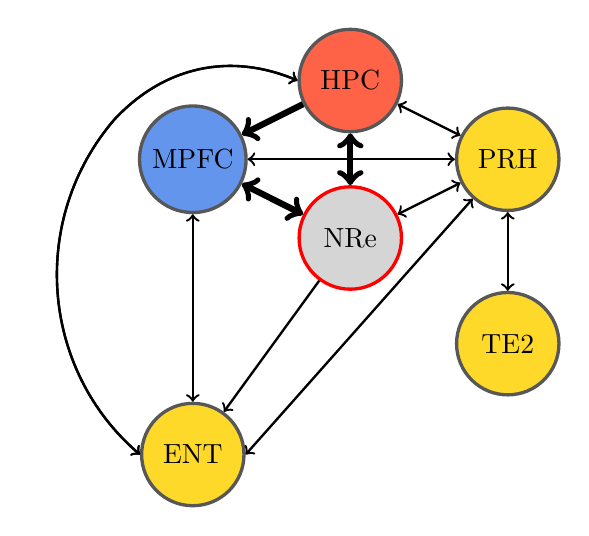
\begin{tikzpicture}[
        roundnode/.style={circle, draw=black!66, very thick, minimum size=7mm}]
        \node[roundnode, minimum size=13mm, fill=myred] at (0, 1) (HPC) {HPC};
        \node[roundnode,minimum size=13mm, fill=gray!33, draw=red] at (0,-1) (NRE) {NRe};
        \node[roundnode,minimum size=13mm, fill=myyellow] at (2,0) (PRH) {PRH};
        \node[roundnode,minimum size=13mm, fill=myblue] at (-2, 0) (MPFC) {MPFC};
        \node[roundnode,minimum size=13mm, fill=myyellow] at (-2, -3.75) (ENT) {ENT};
        \node[roundnode,minimum size=13mm, fill=myyellow] (TE2) [below=of PRH] {TE2};
        \coordinate (top) at (-3,0.5);
        % light lines
        \draw[line width=0.3mm,<->] (PRH) -- (NRE);
        \draw[line width=0.3mm,<->] (PRH) -- (HPC);
        \draw[line width=0.3mm,<->] (ENT) -- (MPFC);
        \draw[line width=0.3mm,<->] (PRH) -- (TE2);
        \draw[line width=0.3mm,<->] (ENT.east) -- (PRH);
        \draw[line width=0.3mm,->] (NRE) -- (ENT);
        \draw[line width=0.3mm,<->] (PRH) -- (MPFC);
         %thick line
        \draw[line width=0.8mm,<->] (NRE) -- (MPFC);
        \draw[line width=0.8mm,<->] (NRE) -- (HPC);
        \draw[line width=0.8mm,->] (HPC) -- (MPFC);
         %curved line
        \path[line width=0.3mm, black, <-] (ENT.west) edge[bend left=45] node [left] {} (top);
        \path[line width=0.3mm, black, ->] (top) edge[bend left=35] node [left] {} (HPC.west);
        \path[line width=0.3mm, black, <-] (ENT.west) edge[bend left=45] node [left] {} (top);
        \path[line width=0.3mm, black, ->] (top) edge[bend left=35] node [left] {} (HPC.west);
        \end{tikzpicture}
\end{document}
